\documentclass[a4paper,9pt]{article}
\usepackage{graphicx}
\usepackage{amsmath}
\usepackage{hyperref}
\usepackage{float}
\usepackage[margin=1in, paperheight=400mm]{geometry}
\usepackage{fontspec}

\graphicspath{{img/}}

\title{\vspace*{-1in}Summary report for Machine Learning}

\author{Magdalena Pakuła \& Jakub Pawlak}

\date{}

\begin{document}

\maketitle


\section{KNN approach}
\subsection{Overview}

Our KNN classifier is parametrized by the number of neighbors $k$, and the distance function, $d$.
When given a list of movies the user has watched, and a new movie to predict, it calculates the distance between the new movie and each of the watched movies, and selects $k$ closest to the new movie.
After that, ratings of all the selected movies is performed to produce a single predicted rating for the new movie.
The aggregation we chose is the review that occurs most often (bincount followed by argmax).

\paragraph{Movie features}
For each movie, we extracted the following data from TMDB:
budget, popularity, release year, revenue, runtime, vote average, vote count, genres, cast, director.

One of the first remarks made was that there are different kinds of features, which we distinguished as follows.
First, there are \emph{scalar} features, which are just numbers, like the revenue or duration.
Second, there are categorical features, which have some set of possible values, and take one of them,
and lastly, there are multi-valued features, like cast of the movie.

Categorical and multi-valued features could be one-hot encoded, however this would create several issues.
Firstly, one-hot encoding requires that all of the possible values are present in the training set.
If there was a new movie that had an actor or director that was not present in the training, there would not be a way to encode it.
Secondly, the number of output dimensions of one-hot encoding depends on the characteristics of input data, which would impact the relative influence of certain features on the total distance (similarity).

For these reasons, we decided to compute distances (similarities) separately, and use their linear combination for a final result, used for comparing movies. Such approach would also allow us to chose diffent measures, based on the data characteristics.

\paragraph{Data Preprocessing}
To prepare the features for similarity calculations, the scalar features were scaled to a range $[0,1]$, using min-max scaler fitted to the entirety of the training data.

\paragraph{Similarity Measures}
The similarity between two movies was computed as a weighted sum of component wise similarities,
using different metrics for various feature types:

\begin{itemize}
	\item \textbf{Scalar features:} The euclidean similarity metric was primarily used for scalar features. Other metrics, such as manhattan and cosine distances, were evaluated for comparison.
	\item \textbf{Categorical Features:} Jaccard similarity measured the overlap between sets (e.g., genres, cast).
	\item \textbf{Rating Similarity:} We also noticed that we can utilize the training dataset and treat movies as similar, if they have similar ratings by different users. Such rating vectors would however contain many empty entries, therefore we used the cosine distance, because it handles such cases well.
\end{itemize}

The resulting of calculating these distances, was a 5-element vector (one for scalar similarity, 3 for genres, cast and directors, and 1 for rating-based similarity).
The resulting measure would be a dot product of this vector with a 5-element weight vector.
The weight vector could be scaled such that all of its elements add up to 1, however this is not a requirement, as it does not distrupt the ordering.
This weight vector would be another hyperparameter of the model, which was experimented with until we found values that worked best.

\subsection{Results}
The results demonstrated that incorporating user rating similarity significantly improved the accuracy of predictions, as it captures shared user preferences. Additionally, the combination of scalar, categorical, and rating-based similarities provided a balanced metric, ensuring that no single feature type dominated the predictions.

The K-Nearest Neighbour (KNN) model was trained on a subset of the dataset, using a combination of numerical and categorical features. The optimal number of neighbors (\texttt{n\_neighbors}) was determined through grid search, achieving the highest accuracy with \( k = 5 \).

Moreover, the testing shown that the model's performance did not vary very much when experimenting with the values of the weight vector, which may suggest that the user's rating does not depend as much on the movie characteristics, as on the user characteristics (e.g.~users give ``generally good'' ratings, regardless of the movie).
Alternatively, it could suggest a problem with the dataset, which is not statistically representative of the whole movie spectrum. As training data, we use the movies that a given user has watched and rated. However, it is a reasonable assumption that the user will generally tend to watch movies that they like. Therefore, both the training set, and by extension, validation set, are representative of movies that the user tends to watch.

\begin{table}[h]
	\centering
	\begin{tabular}{|l|c|c|}
		\hline
		\textbf{Metric}     & \textbf{Training Data} & \textbf{Validation Data} \\ \hline
		Correct predictions & 0.56                   & 0.37                     \\ \hline
		One-off predictions & 0.21                   & 0.31                     \\ \hline
	\end{tabular}
	\caption{Metrics on the Training and Validation Datasets}
	\label{tab:metrics}
\end{table}

\clearpage
\section{Decision Tree Approach}
\subsection{Overview}

The Decision Tree operates by recursively splitting the dataset based on feature values to create
a hierarchical model, aiming to maximize the homogeneity of the resulting subsets.

\paragraph{Splitting criterion}
The key component of a decision tree is what we call a ``choice''. Because of the distinction of different types of movie features, we describe 3 types of choices:
\begin{itemize}
	\item Scalar choice: For numerical features, tests if a value is smaller or larger than a given threshold,
	\item Categorical choice: For categorical features, tests if it is equal to some value from a set of possible values
	\item Set choice: For multi-valued features, tests if the feature set contains some value
\end{itemize}

Each choice is parametrized by one value. At each step when we create the choice node in the tree, we gather a set of all possible choices, which is union over all features, and all values of that feature, of the appropriate choice type parametrized by that value.

\begin{equation}
	\text{Choices} = \bigcup\limits_{f \in F} \bigcup\limits_{v \in M[f]} c_f(v)
\end{equation}
where $F$ is the set of all features, $M[f]$ is the set of all values of feature $f$ in the set of movies $M$,
and $c_f(v)$ is the appropriate choice type for feature $f$, parametrized by value $v$.

From this set of all possible choices, we find the best one using Gini impurity of the resulting sets.
Each choice splits the set of movies $M$ into sets $M^+$ and $M^-$ of movies that respectively passed and failed the test.

The Gini impurity represents the probabilities of miscategorizing items from each class, and is defined as follws:
\begin{equation}
	I_G(p) = 1 - \sum_{i=1}^{k} p_i^2,
\end{equation}

This measure is calculated for each set $M^+$ and $M^-$, and their weighted average is the score of a split.
The best split is one that minimizes this measure.
After choosing the best set, the child nodes are constructed recursively on sets $M^+$ and $M^-$.

\paragraph{Stopping criteria}
There are 2 cases when recursive training is stopped:
\begin{itemize}
	\item Maximum depth is reached
	\item The training set has only one rating --- in which case splitting further would make no sense.
\end{itemize}


An example of a decision tree induced for a specific user is shown in Figure~\ref{fig:decision_tree}, illustrating how user-specific features were leveraged to make predictions.

\begin{figure}[h!]
	\centering
	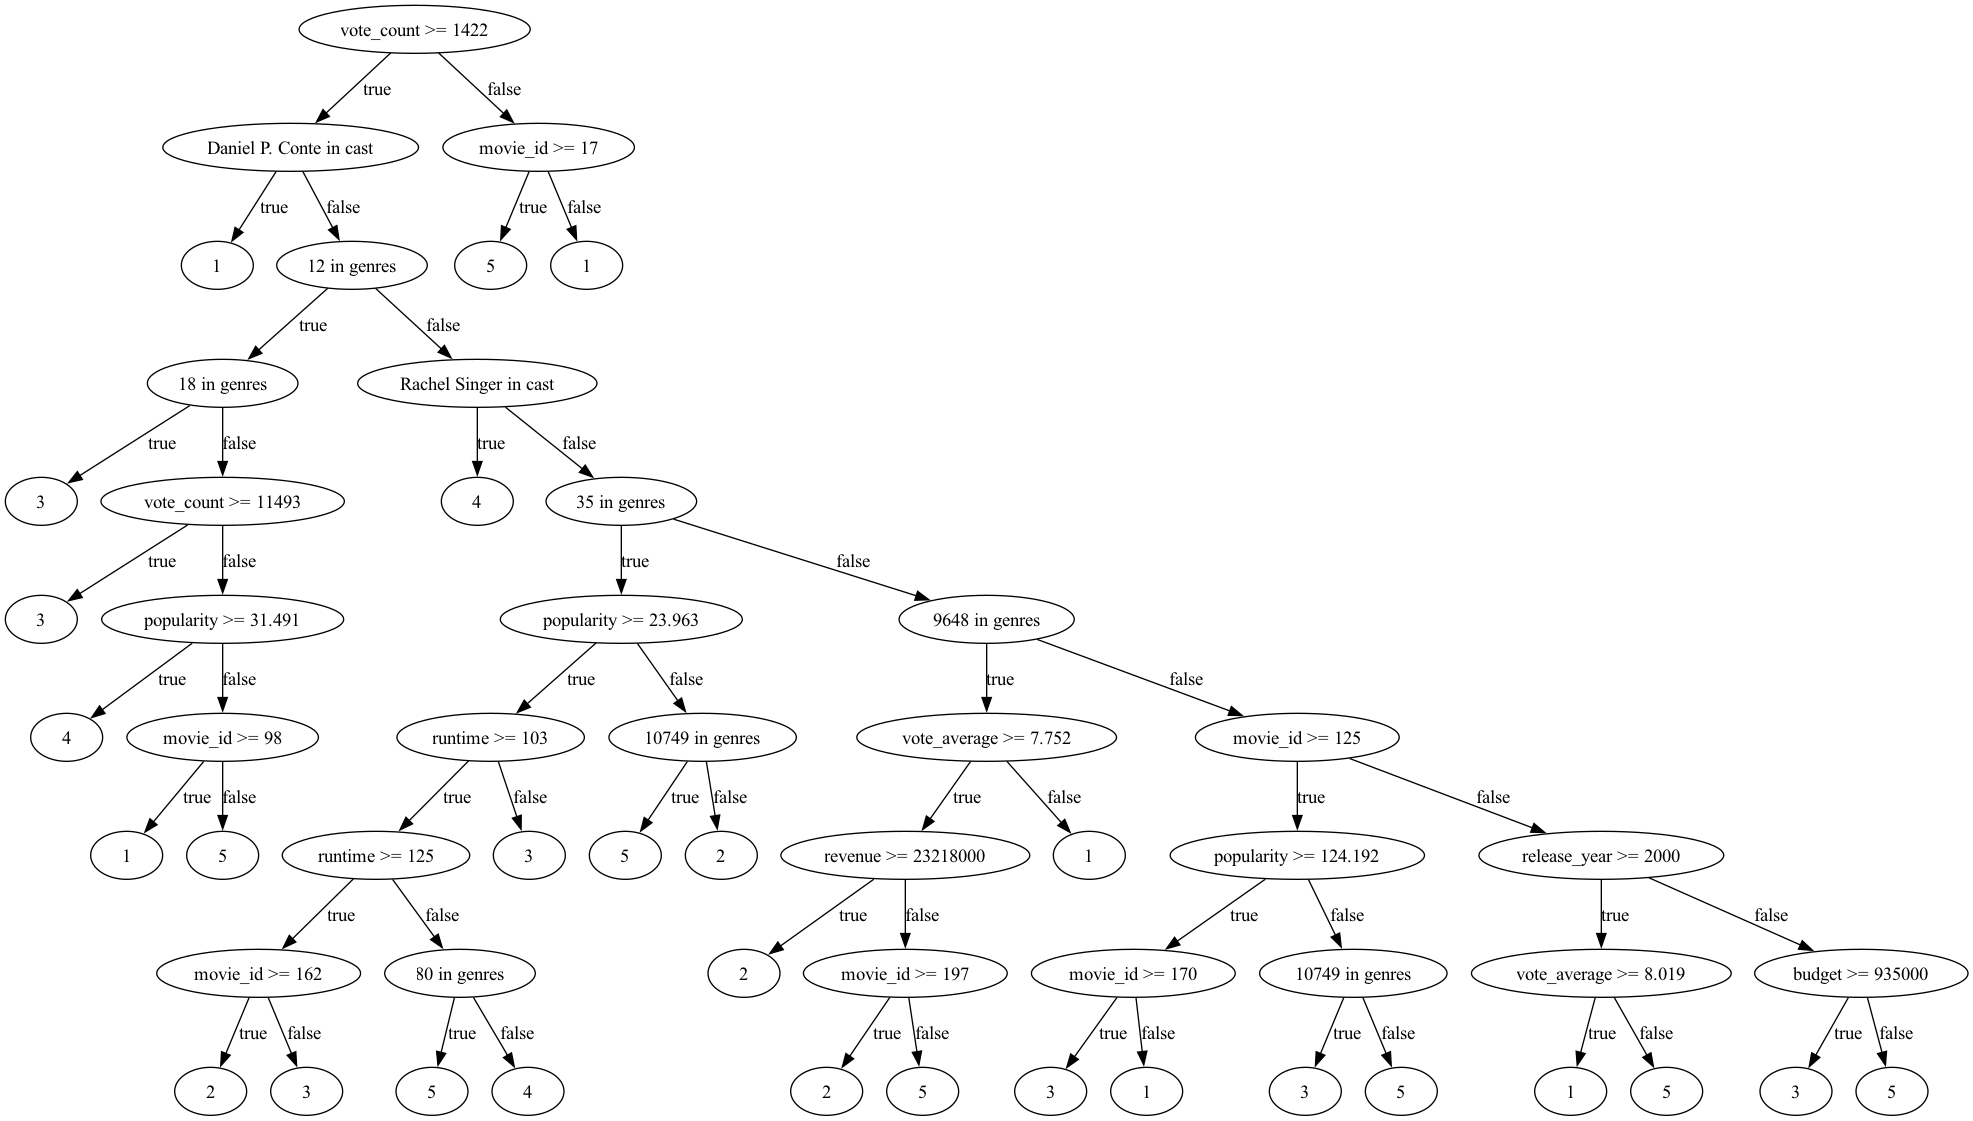
\includegraphics[width=0.4\textwidth]{tree}
	\caption{Visualization of an induced decision tree for a single user.}
	\label{fig:decision_tree}
\end{figure}

\subsection{Results}
The performance metrics indicated:

\begin{table}[ht]
	\centering
	\begin{tabular}{|l|c|c|}
		\hline
		\textbf{Metric}     & \textbf{Training Data} & \textbf{Validation Data} \\ \hline
		Correct predictions & 0.67                   & 0.40                     \\ \hline
		One-off predictions & 0.16                   & 0.29                     \\ \hline
	\end{tabular}
	\caption{Metrics on the Training and Validation Datasets}
	\label{tab:decision_tree_results}
\end{table}

Decision trees demonstrated capability to fit specific user preferences, resulting in scores higher than KNN.
They were able to identify patterns such as disliked actors or favorite genres. Moreover, their underlying representation is easy to reason about.

The drawback of decision trees is that they are prone to overfitting. Even small changes in the training data can completely change the preferred choice of the tree. This makes this model very sensitive to noise or outliers in the training dataset, leading to poor generalization capabilities.

The behavior of the tree is controlled by its depth, which is a hyperparameter of the model.
If the tree is too shallow, it may fail to capture the user's preferences, but if it's too high, the tree might become very sensitive to outliers, which can be seen in the example image, where in the deep nodes, the tree creates braches for specific movies. We chose the depth of our tree by gradually increasing it until the accuracy on the validation dataset stopped increasing.

\clearpage
\section{Random Forest Approach}
\subsection{Overview}
The Random Forest approach is an ensemble learning method that combines multiple decision trees
to enhance predictive performance and reduce overfitting.
By aggregating the predictions of several individual trees, Random Forest mitigates the limitations of
single decision trees, such as sensitivity to noise and high variance.
The ensemble's diversity was assured through two key mechanisms: the random selection of feature
subsets for each tree and the use of bootstrapped training datasets, ensuring that each tree received
a unique perspective on the data.

The Random Forest model was implemented with the
following key components:

\begin{itemize}
	\item \textbf{Random Feature Selection}:
	      A custom class, \texttt{\_RandomFeatureSelector}, was created to randomly select a subset of features for each tree. This ensured that individual trees focused on different attributes of the data, reducing the correlation between trees in the ensemble. For example, features like \texttt{budget}, \texttt{genres}, and \texttt{popularity} were considered, while identifiers such as \texttt{title} were excluded to enhance generalization.
	\item \textbf{Bootstrapping}:
	      To further ensure diversity, bootstrapped training datasets were generated by sampling movies with replacement from the original dataset. Each bootstrapped sample included selected features and their corresponding ratings.
	\item \textbf{Binary Decision Trees}:
	      Each decision tree in the Random Forest was built using binary splits, where node conditions were satisfied or not. The maximum tree depth was restricted to 5 to balance computational efficiency and model expressiveness. The trees were trained to optimize the Gini impurity at each split, ensuring effective feature selection during induction.
	\item \textbf{Aggregation of Predictions}:
	      The Random Forest model combined the predictions of all trees in the ensemble using an averaging function. This aggregation reduced the variance of individual predictions and improved the robustness of the final recommendation scores.
\end{itemize}


These principles collectively ensure that the Random Forest model reduces overfitting while maintaining high predictive accuracy.

Since decision trees are interpretable models, it is possible to visualize the decision-making process of individual trees within the Random Forest. Figure~\ref{fig:random_forest_trees} illustrates sample decision trees from the ensemble for a single user. Each tree captures a unique hierarchical structure based on feature thresholds, contributing to the ensemble's diversity.
The first tree reflects preferences based on actors and release year, the second one --- popularity, revenue, and budget, and the last one --- genres, budget and directors.

\begin{figure}[h!]
	\centering
	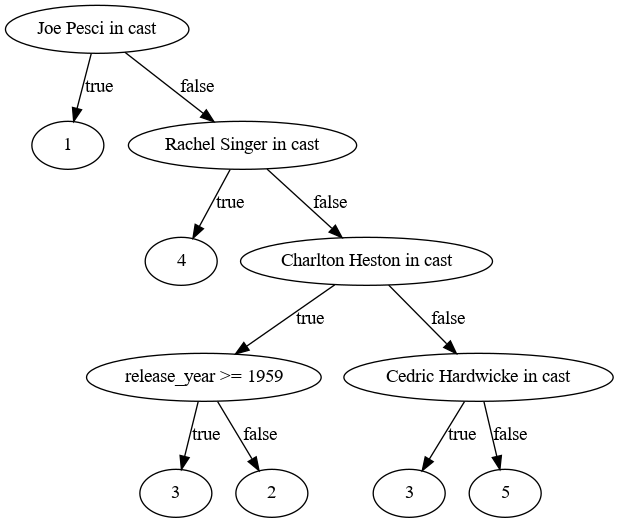
\includegraphics[width=0.25\textwidth]{forest/tree_0.png}
	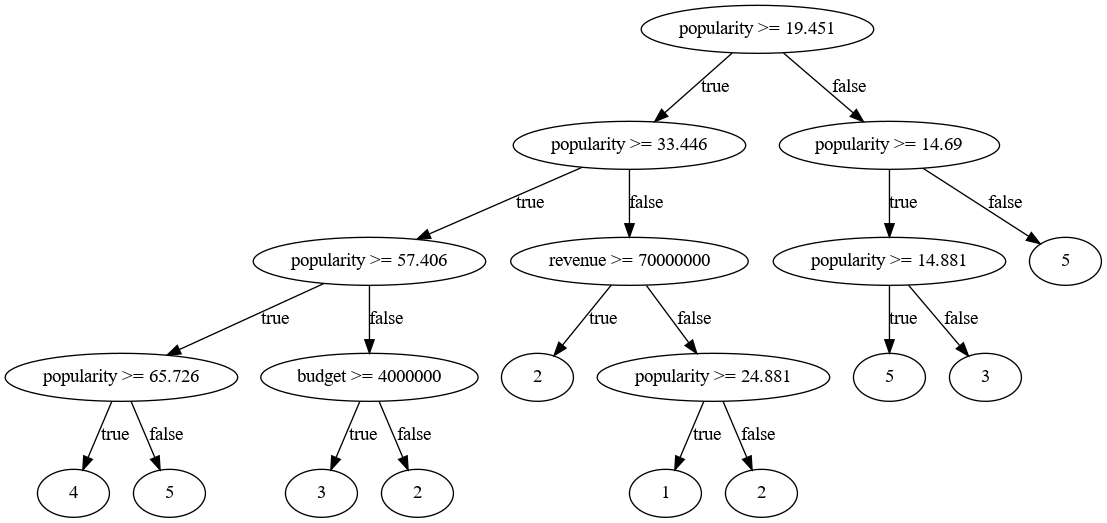
\includegraphics[width=0.25\textwidth]{forest/tree_9.png}
	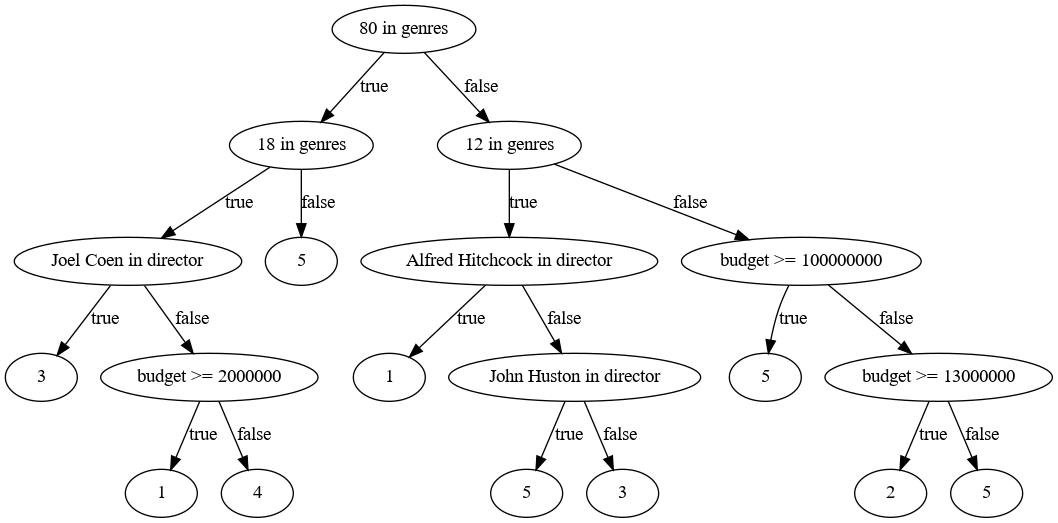
\includegraphics[width=0.25\textwidth]{forest/tree_4.png}
	\caption{Sample decision trees from the Random Forest ensemble for a single user. Each tree reflects a unique subset of features and bootstrapped training data.}
	\label{fig:random_forest_trees}
\end{figure}

\subsection{Results}
The performance metrics indicated:

\begin{table}[ht]
	\centering
	\begin{tabular}{|l|c|c|}
		\hline
		\textbf{Metric}     & \textbf{Training Data} & \textbf{Validation Data} \\ \hline
		Correct predictions & 0.49                   & 0.36                     \\ \hline
		One-off predictions & 0.37                   & 0.40                     \\ \hline
	\end{tabular}
	\caption{Metrics on the Training and Validation Datasets}
	\label{tab:random_forest_results}
\end{table}

Surprisingly the random forest approach did not outperform the decision tree as expected.
We can notice however that the random forest did not have as much drop from training set to validation set performance.
This suggests that is is overfitting less, as expected.

Although it has lower correct prediciton rates, it outperforms the decision tree in the one-off errors, suggesting that it did sacrifice some exact prediction capabilities for more consistent near-accurate predictions. This may suggest that overall the random forest approach is more robust than a single decision tree.

Another reason might be the wrong choice of hyperparameters. Decision tree has only one, but random forest in addition to the depth of the trees has the number of trees, the way of choosing features and bootstrapping the data, and finally, the aggregation function. This increased number of hyperparameters makes it much more difficult to perform an exhaustive grid search. This is additionally amplified by the fact that random forest is much more computationally intensive that a single decision tree by at least the factor of number of trees.

\clearpage
\section{Person Similarity Approach}
\subsection{Overview}
The Person Similarity approach was employed to predict user ratings for movies by leveraging the similarity
between users based on their historical ratings.
The primary goal was to identify users with similar movie preferences and use their ratings to estimate
the target user's missing ratings.
This approach exclusively considers user evaluations, disregarding movie-specific features, and focuses
on users who have rated the same movies as the target user.

The methodology for similarity measure involved the combination of \textbf{Pearson correlation} and \textbf{Cosine similarity}:

\begin{itemize}
	\item \textbf{Pearson Correlation:} Captures the linear relationship between two users' ratings, centering around their respective mean ratings to account for rating biases.
	      \begin{equation}
		      \operatorname{sim}_\text{pearson}(x,y) = \frac{\sum_{i} (x_i - \bar{x})(y_i - \bar{y})}{\sqrt{\sum_{i} (x_i - \bar{x})^2 \sum_{i} (y_i - \bar{y})^2}},
	      \end{equation}
	      where \( x_i \) and \( y_i \) are ratings given by two users for the same movies, and \( \bar{x} \), \( \bar{y} \) are their respective mean ratings.

	\item \textbf{Cosine Similarity:} Evaluates the angular similarity between two users' rating vectors, ignoring the magnitude of their ratings:
	      \begin{equation}
		      \operatorname{sim}_\text{cosine}(x,y) = \frac{\sum_{i} x_i y_i}{\sqrt{\sum_{i} x_i^2} \sqrt{\sum_{i} y_i^2}}.
	      \end{equation}
\end{itemize}


A weighting factor, $w$, was used to blend the two metrics:
\begin{equation}
	\operatorname{sim}(x,y) = w \cdot \operatorname{sim}_\text{pearson}(x,y) + (1 - w) \cdot \operatorname{sim}_\text{cosine}(x,y) .
\end{equation}
This approach allowed flexibility in prioritizing either metric based on the validation performance.

To mitigate the influence of users with very few overlapping ratings, a damping factor was applied, scaling down the
similarity score when the number of shared ratings was low.

For efficiency, computed similarity scores were cached in a dictionary, avoiding redundant calculations when the same user
pairs were compared multiple times.

To predict the target user's rating for a specific movie, only users who had rated the target movie and shared common
rated movies with the target user were considered for prediction.

The predicted rating, \( \hat{r}_{u,m} \), was calculated using a weighted average of ratings from similar users:
\begin{equation}
	\hat{r}_{u,m} = \frac{\sum_{v \in N(m)} sim(u,v) \cdot r_{v,m}}{\sum_{v \in N(m)} |sim(u,v)|},
\end{equation}
where \( \hat{r}_{u,m} \) is the predicted rating for user \( u \) on movie \( m \), \( sim(u,v) \) is the similarity score between user \( u \) and user \( v \), and \( r_{v,m} \) is the rating given by user \( v \) to movie \( m \). \( N(m) \) denotes the set of users who have rated movie \( m \).

In cases where insufficient overlapping ratings were available, predictions defaulted to the target user's global average rating for better generalization.

\subsection{Results}
The performance metrics indicated:

\begin{table}[ht]
	\centering
	\begin{tabular}{|l|c|c|}
		\hline
		\textbf{Metric}     & \textbf{Training Data} & \textbf{Validation Data} \\ \hline
		Correct predictions & 0.34                   & 0.32                     \\ \hline
		One-off predictions & 0.49                   & 0.46                     \\ \hline
	\end{tabular}
	\caption{Metrics on the Training and Validation Datasets}
	\label{tab:person_similarity_results}
\end{table}

The Person Similarity approach demonstrated a strong ability to predict user ratings,
particularly in scenarios where users had rated a substantial number of common movies.
However, its performance was more limited when the overlap of rated movies was small, as the approach relies heavily
on the availability of common ratings for comparison.

In conclusion, while the Person Similarity approach provides an effective method for movie rating prediction based on user
similarities, its performance can be impacted by the sparsity of the rating matrix.
Nonetheless, it remains a valuable technique for collaborative filtering in recommender systems.

\clearpage
\section{Collaborative Filtering Approach}
Collaborative filtering is a method used for making automatic predictions about the interests of a user by collecting preferences or taste information from many users. This approach assumes that if a user has agreed with another user on one issue, they are likely to agree on other issues as well.

\subsection{Overview}
This model was trained using a matrix factorization technique, where the user-item interaction matrix (ratings) was decomposed into two lower-dimensional matrices: one representing user parameters and the other representing movie features. This approach allows the model to learn latent factors that explain user preferences and movie characteristics.

\paragraph{Dimensionality Selection}
In our implementation, we initialized the feature space with a dimensionality of 15. This choice was based on empirical testing, balancing model complexity and performance. A higher dimensionality can capture more nuanced patterns but may lead to overfitting. Therefore, we monitored performance metrics on the training set and adjusted dimensionality as necessary to optimize generalization.

\paragraph{Generalization Methods}
To ensure that the model generalizes well to unseen data, several techniques were employed:

\begin{itemize}
	\item \textbf{Regularization}: Both the user and movie feature matrices were subjected to regularization to prevent overfitting. The regularization parameter is denoted as \( \lambda \), and it is applied as follows:
	      \begin{equation}
		      L = \sum_{u=1}^{U} \sum_{m=1}^{M} \left( \hat{y}(m,u) - y(m,u) \right)^2 + \lambda \left( \|P\|^2 + \|X\|^2 \right) \tag{1}
	      \end{equation}
	      where \(P\) and \(X\) represent the user and movie feature matrices, respectively.

	\item \textbf{Mean Normalization}: Prior to training, mean normalization was applied to the ratings. This involves centering the ratings around zero:
	      \begin{equation}
		      \bar{y}_m = \frac{1}{U} \sum_{u=1}^{U} y(m,u) \tag{2}
	      \end{equation}
	      The normalized ratings are given by:
	      \begin{equation}
		      y'_{m,u} = y_{m,u} - \bar{y}_m \tag{3}
	      \end{equation}

	\item \textbf{Validation and Cross-Validation}: To assess the model’s generalization abilities, we employed \( k \)-fold cross-validation (with \( k = 5 \)). The process involves splitting the dataset into \( k \) subsets and iteratively training and validating the model on different combinations of these subsets.
\end{itemize}

\paragraph{Algorithm Implementation}
Our implementation details for the collaborative filtering model are as follows:

\subparagraph{Movie Ratings}
Let \( y_{m,u} \), or alternatively \( y[m,u] \), denote the rating of movie \( m \) by user \( u \). Therefore, \( y \) will be an \( M \times U \) matrix:
\begin{equation}
	y =
	\begin{bmatrix}
		y_{1,1} & y_{1,2} & \cdots & y_{1,U} \\
		y_{2,1} & y_{2,2} & \cdots & y_{2,U} \\
		\vdots  & \vdots  & \ddots & \vdots  \\
		y_{M,1} & y_{M,2} & \cdots & y_{M,U}
	\end{bmatrix} \tag{4}
\end{equation}
Valid ratings are integers from 0 to 5. If \( y_{m,u} \) takes the value of NaN, it denotes that user \( u \) did not rate movie \( m \).

\subparagraph{Movie Features}
Let \( N \) be the total number of features. Then, \( x_{m,n} \) will be the \( n \)-th feature of the movie \( m \). As such, \( x \) will be an \( M \times N \) matrix:
\begin{equation}
	x =
	\begin{bmatrix}
		x_{1,1} & x_{1,2} & \cdots & x_{1,N} \\
		x_{2,1} & x_{2,2} & \cdots & x_{2,N} \\
		\vdots  & \vdots  & \ddots & \vdots  \\
		x_{M,1} & x_{M,2} & \cdots & x_{M,N}
	\end{bmatrix} \tag{5}
\end{equation}

\subparagraph{User Parameters}
Each user \( u \) will have a set of parameters \( p_u \) corresponding to the movie features, plus one additional feature \( p_{u,0} \):
\begin{equation}
	p =
	\begin{bmatrix}
		p_{1,0} & p_{1,1} & p_{1,2} & \cdots & p_{1,N} \\
		p_{2,0} & p_{2,1} & p_{2,2} & \cdots & p_{2,N} \\
		\vdots  & \vdots  & \vdots  & \ddots & \vdots  \\
		p_{U,0} & p_{U,1} & p_{U,2} & \cdots & p_{U,N}
	\end{bmatrix} \tag{6}
\end{equation}

\paragraph{Calculating Predictions}
The predicted rating of movie \( m \) by user \( u \) will be denoted as \( \hat{y}(m,u) \). It will be calculated as follows:
\begin{equation}
	\hat{y}(m,u) = p_{u,0} + \sum_{n=1}^N p_{u,n} \cdot x_{m,n} \tag{7}
\end{equation}
Alternatively, as a dot product:
\begin{equation}
	\hat{y}(m,u) = p_{u,0} + p[u,1:] \cdot x[m,:] \tag{8}
\end{equation}
where
\begin{equation}
	p[u,1:] = \begin{bmatrix}
		p_{u,1} & p_{u,2} & \cdots & p_{u,N}
	\end{bmatrix}, \tag{9}
\end{equation}
and
\begin{equation}
	x[m,:] = \begin{bmatrix}
		x_{m,1} & x_{m,2} & \cdots & x_{m,N}
	\end{bmatrix}. \tag{10}
\end{equation}

\paragraph{Calculating Errors}
The error function will be as follows:
\begin{equation}
	Q(p,x) = \frac{1}{2} \sum_{m,u : y[m,u] \neq -1} (\hat{y}(m,u) - y[m,u])^2 \tag{11}
\end{equation}

\paragraph{Partial Derivatives}
\subparagraph{Zeroth User Parameter}
\begin{equation}
	\frac{\partial Q}{\partial p_{u,0}} = \sum_{m : y[m,u] \neq -1} (\hat{y}[m,u] - y[m,u]) \tag{12}
\end{equation}

\subparagraph{Other User Parameters (\(1, \ldots, N\))}
\begin{equation}
	\frac{\partial Q}{\partial p_{u,n}} = \sum_{m : y[m,u] \neq -1} (\hat{y}[m,u] - y[m,u]) \cdot x[m,n] \tag{13}
\end{equation}

\subparagraph{Movie Parameters}
\begin{equation}
	\frac{\partial Q}{\partial x_{m,n}} = \sum_{u : y[m,u] \neq -1} (\hat{y}[m,u] - y[m,u]) \cdot p[u,n] \tag{14}
\end{equation}

The collaborative filtering approach demonstrated promising results in predicting user ratings for movies. The training process involved iterating over multiple epochs and adjusting the parameters based on the computed gradients. The loss function focused on minimizing the difference between predicted and actual ratings, defined as:
\begin{equation}
	Q(P, X) = \frac{1}{2} \sum_{m,u : y(m,u) \neq \text{NaN}} \left( \hat{y}(m,u) - y(m,u) \right)^2 \tag{15}
\end{equation}
\subsection{Results}
The training phase achieved a stable loss value after multiple iterations.
The following metrics were used to evaluate performance:

\begin{table}[h]
	\centering
	\begin{tabular}{|l|c|c|}
		\hline
		\textbf{Metric}     & \textbf{Training Data} & \textbf{Validation Data} \\ \hline
		Correct Predictions & 0.54                   & 0.38                     \\ \hline
		One-Off Predictions & 0.39                   & 0.38                     \\ \hline
	\end{tabular}
	\caption{Performance Metrics on Training and Validation Datasets}
	\label{tab:predictions_metrics}
\end{table}

The model was validated on a separate dataset to assess its ability to generalize.
Cross-validation techniques (e.g., \(k\)-fold cross-validation with \(k=5\)) were employed to mitigate variance due to data partitioning.
These results demonstrate the effectiveness of the collaborative filtering approach, with a balance between
fitting the training data and generalizing to unseen data.

\clearpage
\section{Summary and Comparison}

\begin{itemize}
	\item Summarize the results for all approaches using test data or feedback.
	\item Compare performance metrics and discuss the strengths and weaknesses of each method.
	\item{} [Include a table or graph for comparison, if applicable].
\end{itemize}
\end{document}
